\documentclass[final,5p,times,twocolumn]{elsarticle}

\usepackage{amsmath,amssymb,amsfonts}
\usepackage{graphicx}
\usepackage{booktabs}
\usepackage{hyperref}
\usepackage{lineno}
\usepackage{microtype}
\usepackage{siunitx}
\usepackage{tabularx}

\journal{SoftwareX}

\begin{document}

\begin{frontmatter}

\title{SimuPharm: An Open-Source Multi-Instrument Analytical and Spectroscopic Simulation Suite for Pharmaceutical Research and Education}

\author[inst1]{SimuPharm Development Team\corref{cor1}}
\ead{info@simupharm.io}

\cortext[cor1]{Corresponding author. Permanent repository: \url{https://github.com/simupharm/simupharm}}
\affiliation[inst1]{organization={SimuPharm Open Source Project, Independent Computational Chemistry Group},
            country={International}}

\begin{abstract}
Analytical instrument training and method optimization in pharmaceutical chemistry frequently encounter prohibitive obstacles: high operational expenditures, consumable solvent costs, hazardous waste generation, and competitive access bottlenecks for advanced hardware such as High-Performance Liquid Chromatography (HPLC), Fourier-Transform Infrared (FTIR), and Mass Spectrometry (MS). While single-technique pedagogical simulators exist, no unified, high-throughput, open-source Python library currently integrates multiple orthogonal pharmaceutical analytical instruments with chemometric cross-validation into an extensible programmatic environment.

In this work, we introduce \textbf{SimuPharm}, an open-source Python library and simulation suite that models seven primary analytical and spectroscopic instruments: (1) HPLC with Van Deemter column kinetics, capacity factors, peak tailing asymmetry, and United States Pharmacopeia (USP $\langle$621$\rangle$) system suitability; (2) UV-Vis spectrophotometry with Beer-Lambert absorption, Gaussian band deconvolution, and ICH Q2(R1) calibration statistics (LOD/LOQ); (3) FTIR spectroscopy with Michelson interferogram Fast Fourier Transforms (FFT), transmittance modeling, and automated functional group correlation tagging; (4) Gas Chromatography (GC) with Golay capillary plate kinetics and multi-ramp linear temperature programming; (5) Electron Ionization (EI) and Electrospray Ionization (ESI) Mass Spectrometry with natural isotopic envelope calculations (M, M+1, M+2) and fragmentation trees; (6) Polarimetry with Biot's law, Drude wavelength dispersion, and enantiomeric excess ($ee$) determination; and (7) Particle Size Analysis (PSA) with dynamic light scattering, log-normal size distribution, D10/D50/D90 percentile calculations, and span metrics. Built on pure Python, NumPy, and SciPy, SimuPharm achieves sub-5-millisecond execution times per run, supports headless batch computational pipelines, and provides orthogonal spectral cross-matching across a curated database of 21 pharmacopeial active pharmaceutical ingredients (APIs). SimuPharm offers an accessible, zero-cost, environmentally sustainable platform for pharmaceutical method development, computational screening, and virtual laboratory education.
\end{abstract}

\begin{keyword}
Pharmaceutical Analysis \sep Chromatography Simulation \sep Spectroscopy Modeling \sep Van Deemter Equation \sep Chemometrics \sep Virtual Laboratory \sep Open-Source Software
\end{keyword}

\end{frontmatter}

\section*{Current code version}
An overview of the code metadata is presented in Table~\ref{tab:metadata}.

\begin{table*}[t]
\caption{Code metadata description}
\label{tab:metadata}
\small
\begin{tabularx}{\textwidth}{l p{5.5cm} X}
\toprule
\textbf{Nr.} & \textbf{Code metadata description} & \textbf{Metadata details} \\
\midrule
C1 & Current code version & v1.0.0 \\
C2 & Permanent link to code / repository & \url{https://github.com/simupharm/simupharm} \\
C3 & Permanent link to reproducible release & \url{https://github.com/simupharm/simupharm/releases/tag/v1.0.0} \\
C4 & Legal Code License & MIT License \\
C5 & Code versioning system used & Git \\
C6 & Software code language & Python 3.10+ \\
C7 & Compilation requirements \& dependencies & \texttt{numpy >= 1.22.0}, \texttt{scipy >= 1.8.0}, \texttt{pydantic >= 2.0.0} \\
C8 & Optional dependencies & \texttt{matplotlib >= 3.5.0} (visualization), \texttt{pytest >= 7.0.0} (test suite) \\
C9 & Supported operating systems & Linux (Ubuntu, Debian, CentOS, Fedora), macOS, Windows 10/11 \\
C10 & Support contact email & \url{info@simupharm.io} \\
\bottomrule
\end{tabularx}
\end{table*}

\section{Motivation and Significance}
\label{sec:motivation}

Modern pharmaceutical quality assurance, regulatory compliance, and drug discovery rely on an extensive battery of complementary analytical instrumentation. Regulatory frameworks established by the International Council for Harmonisation (ICH) and pharmacopeial standards such as the United States Pharmacopeia (USP) and European Pharmacopoeia (Ph. Eur.) require rigorous chemical identification, assay quantitation, purity assessment, and chromatographic system suitability validation~\cite{ich2005q2,usp2020chapter621}. However, delivering hands-on training and conducting iterative method development across these instruments face substantial practical constraints:

\begin{enumerate}
    \item \textbf{Capital and Maintenance Costs:} Modern analytical platforms---such as ultra-high-performance liquid chromatographs (UHPLC) coupled to triple-quadrupole mass spectrometers---represent capital investments frequently exceeding \$100,000 to \$300,000 USD, accompanied by substantial service contracts, expensive chromatographic columns, and specialized deuterium lamp replacements~\cite{snyder2010modern}.
    \item \textbf{Consumable Consumption and Environmental Footprint:} Traditional chromatographic method development involves extensive trial-and-error solvent screening, consuming significant volumes of toxic, volatile organic solvents (such as acetonitrile, methanol, and hexane). In alignment with Green Analytical Chemistry (GAC) principles, computational pre-optimization dramatically mitigates chemical waste and carbon footprint~\cite{galuszka2013principles}.
    \item \textbf{Instrument Access Bottlenecks and Risk of Hardware Damage:} In academic instruction, student-to-instrument ratios frequently exceed 15:1, forcing students into passive observation rather than active, exploratory trial-and-error experimentation. Furthermore, novice learners risk catastrophic column overpressurization, stationary phase precipitation, or detector burn-out during unconstrained exploration~\cite{bosch2021virtual}.
    \item \textbf{Fragmentation of Existing In Silico Tools:} While individual standalone software tools exist for single techniques (e.g., commercial packages like DryLab for HPLC or ACD/Labs for NMR/UV), they are typically proprietary, cost-prohibitive, platform-locked, and lack a unified, scriptable API. Prior open-source simulators are overwhelmingly restricted to single standalone instruments, lack programmatic Python bindings, or omit standardized pharmacopeial suitability calculations.
\end{enumerate}

To address this methodological and educational gap, we developed \textbf{SimuPharm}, an open-source, lightweight, multi-instrument simulation suite designed from the ground up to provide: (a) a unified, physically consistent mathematical foundation across seven core analytical instruments; (b) deterministic, high-throughput in silico method screening capable of running thousands of experimental condition permutations in seconds; (c) built-in pharmacopeial system suitability (USP $\langle$621$\rangle$) and analytical validation metrics (ICH Q2(R1)); (d) an orthogonal multimodal chemometric engine capable of fusing UV-Vis, FTIR, and Mass Spectrometry data to resolve identity ambiguities; and (e) complete open-source availability under the MIT License, with zero commercial dependencies.

\section{Software Description}
\label{sec:description}

\subsection{Software Architecture}
SimuPharm is engineered as a modular, pure-Python library organized into decoupled subpackages: \texttt{simupharm.core} (common base data types), \texttt{simupharm.instruments} (7 physical simulation engines), \texttt{simupharm.database} (21-API curated reference knowledgebase), and \texttt{simupharm.analytics} (chemometric matching and suitability engines). The overall architecture and functional pipeline are depicted in Figure~\ref{fig:architecture}.

\begin{figure*}[!t]
\centering
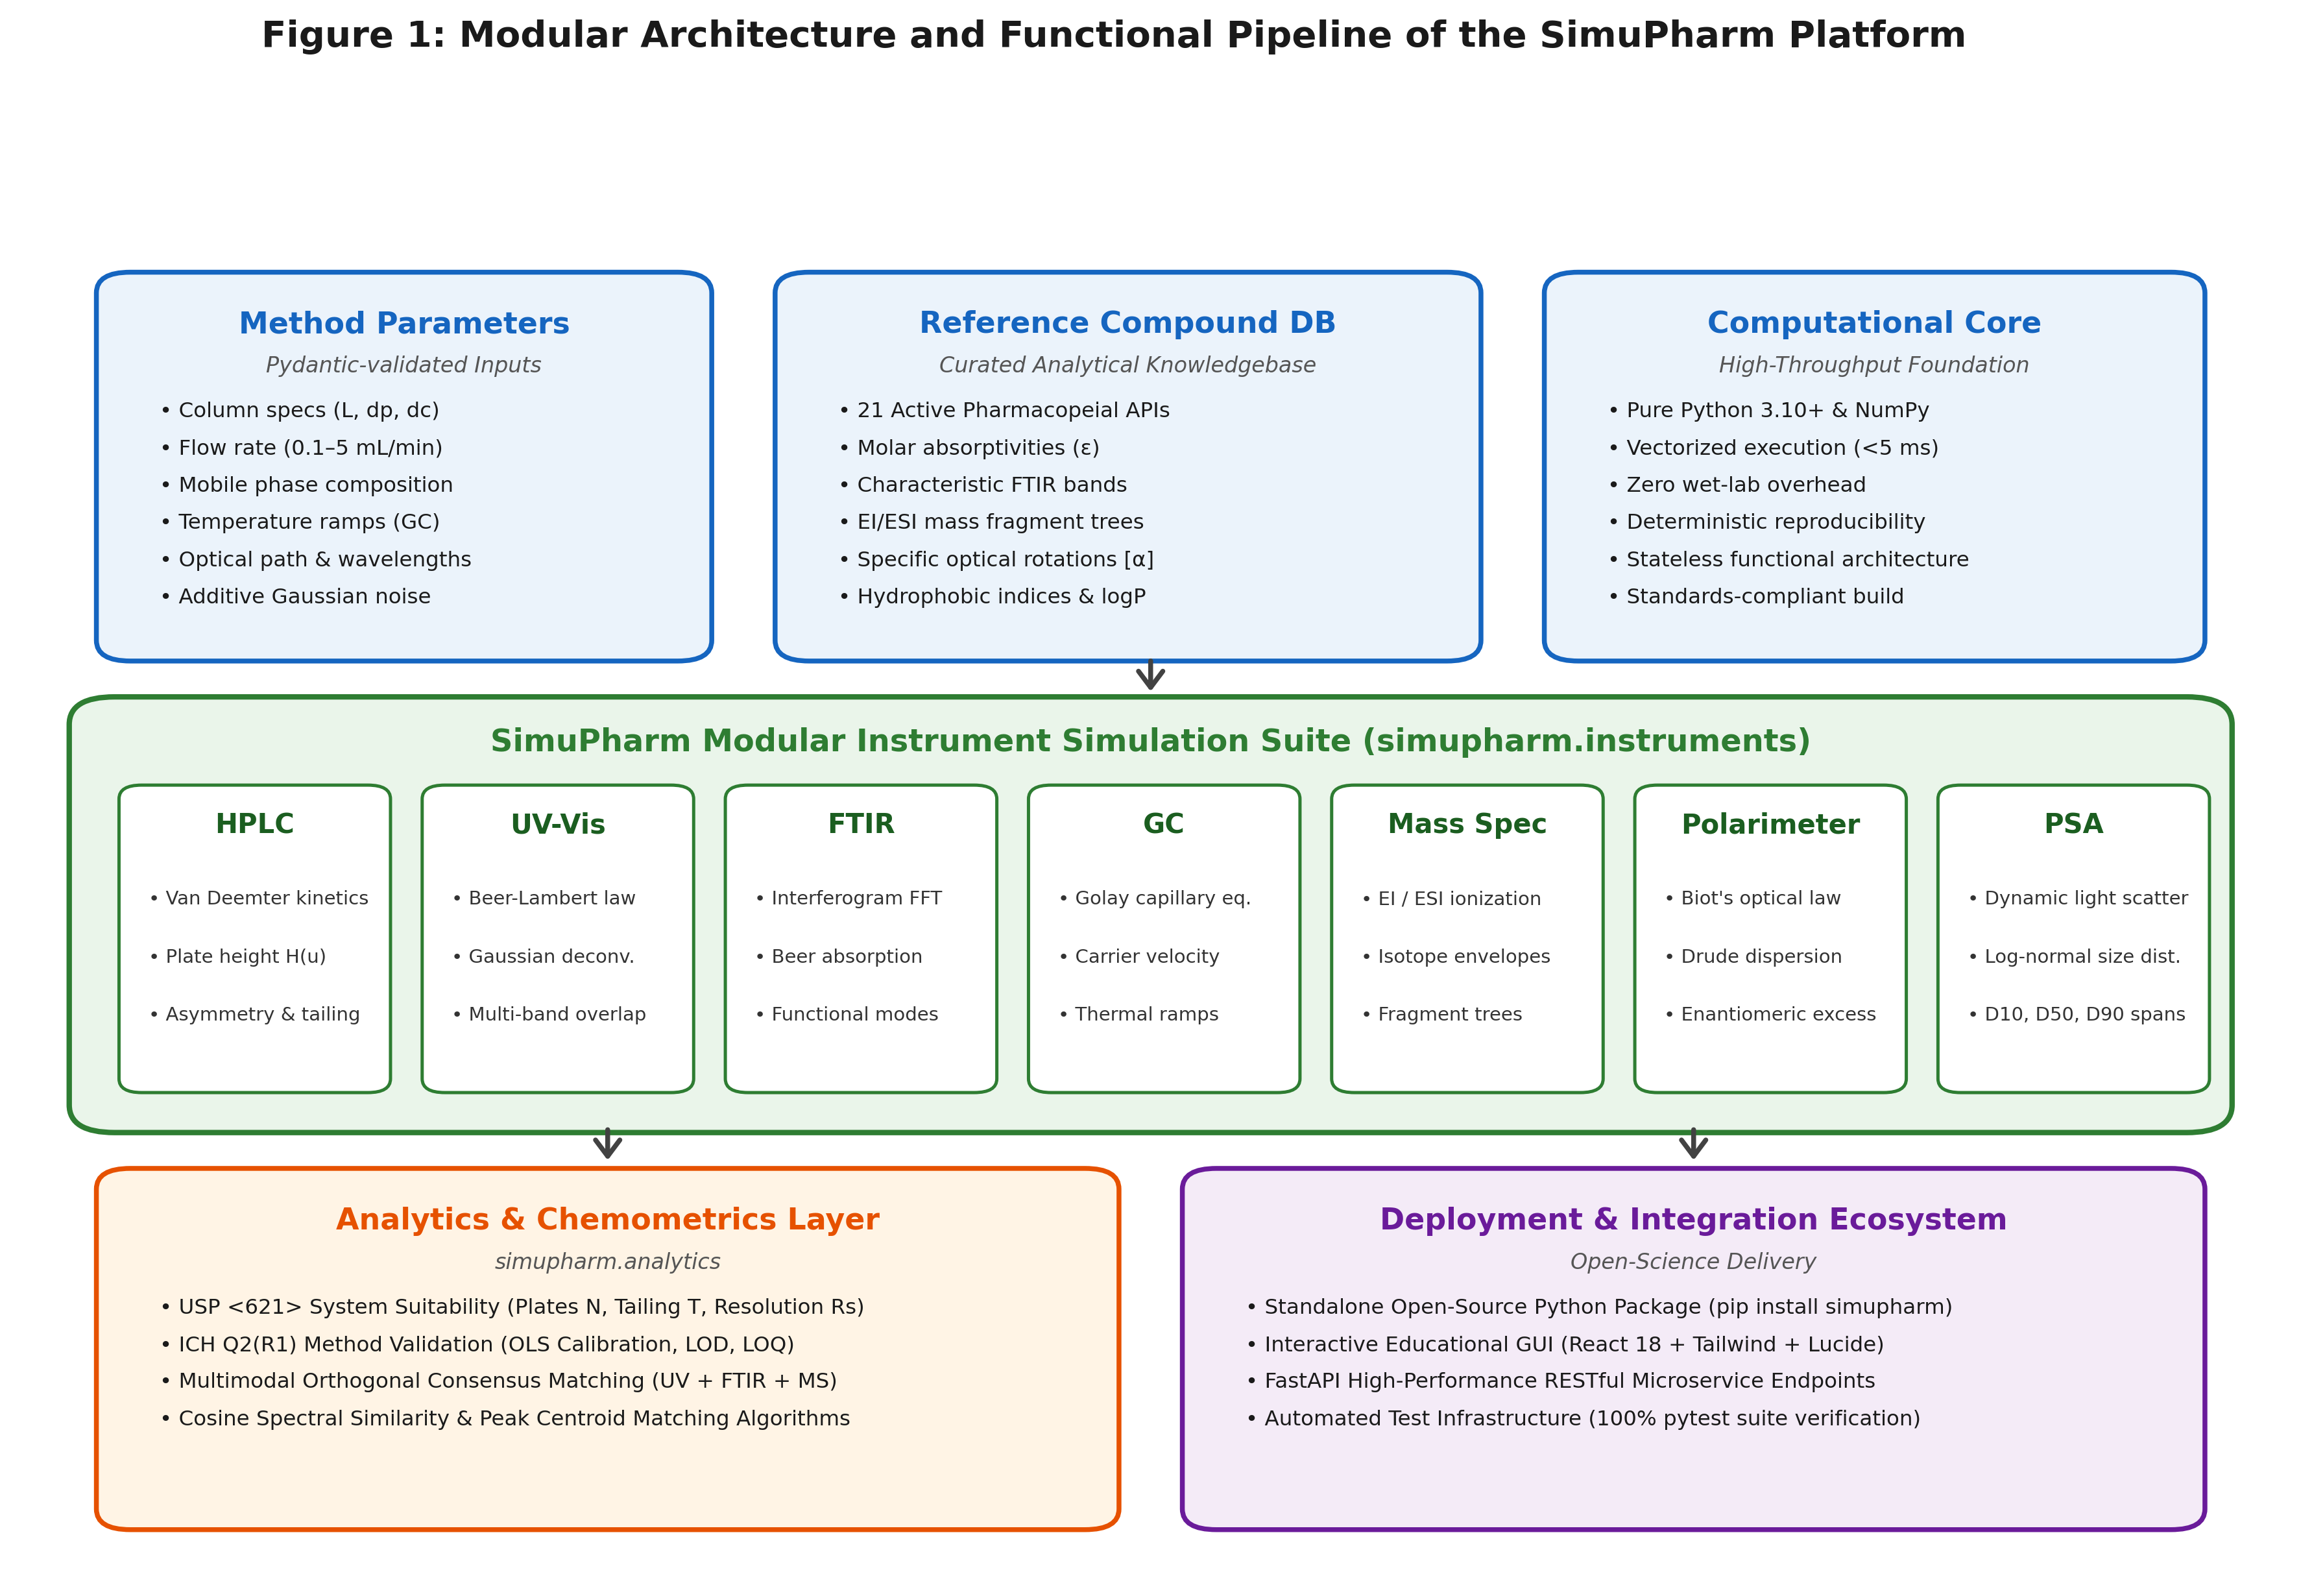
\includegraphics[width=\textwidth]{figures/fig1_system_architecture.png}
\caption{Modular architecture and functional pipeline of the SimuPharm platform. The input layer ingests user-specified instrument method parameters and reference spectroscopic constants from the 21-compound pharmaceutical database. The computation core vectorizes execution across seven analytical instrument engines, delivering physical spectra and chromatograms to the chemometrics layer for USP $\langle$621$\rangle$ suitability and multimodal identification.}
\label{fig:architecture}
\end{figure*}

\subsection{Mathematical Engines and Physical Principles}

\subsubsection{High-Performance Liquid Chromatography (HPLC)}
Separation dynamics are governed by the classic Van Deemter plate height equation~\cite{vandeemter1956longitudinal}:
\begin{equation}
H = A + \frac{B}{u} + C \cdot u
\end{equation}
where $A = 2 \lambda d_p$ accounts for eddy diffusion, $B = 2 \gamma D_m$ represents longitudinal molecular diffusion, $C$ quantifies mass transfer resistance between stationary and mobile phases, and $u$ is mobile phase linear velocity. Theoretical plate count $N$ and dead time $t_0$ are computed from column dimensions ($L, d_c$) and flow rate $F$:
\begin{equation}
N = \frac{L}{H}, \quad t_0 = \frac{\pi (d_c/2)^2 L \epsilon_t}{F}
\end{equation}
Compound retention times $t_R$ are adjusted by the organic modifier percentage ($\%B$) using a modified Snyder-Soczewinski solvent strength relationship:
\begin{equation}
k'_{\text{adj}} = k'_0 \cdot \left(\frac{100 - \%B}{40}\right), \quad t_R = t_0 \cdot (1 + k'_{\text{adj}})
\end{equation}
Peak shapes are synthesized via Gaussian convolution with an exponential decay tailing factor $\tau$ to reproduce realistic column peak asymmetry ($A_s \approx 1.15$):
\begin{equation}
S(t) = \frac{R}{\sigma \sqrt{2\pi}} \exp\left(-\frac{(t - t_R)^2}{2\sigma^2}\right) \cdot \exp\left(-\alpha (t - t_R)\right)
\end{equation}
Chromatographic resolution between consecutive peaks is evaluated per USP $\langle$621$\rangle$:
\begin{equation}
R_s = \frac{2 (t_{R,2} - t_{R,1})}{w_1 + w_2}
\end{equation}

\subsubsection{Ultraviolet-Visible Spectrophotometry (UV-Vis)}
Absorbance follows the Beer-Lambert law across multicomponent mixtures with Gaussian vibronic band profiles~\cite{skoog2017principles}:
\begin{equation}
A(\lambda) = \sum_{i} \epsilon_i \cdot c \cdot l \cdot \exp\left(-\frac{(\lambda - \lambda_{\max,i})^2}{2 \sigma_i^2}\right) + \mathcal{N}(0, \sigma_{\text{noise}}^2)
\end{equation}
Transmittance is derived as $T(\%) = 10^{-A(\lambda)} \times 100\%$. The module provides automated Ordinary Least Squares (OLS) regression across calibration standard series, calculating the coefficient of determination $R^2$, Limit of Detection ($\text{LOD} = 3.3 \sigma_y / S$), and Limit of Quantitation ($\text{LOQ} = 10 \sigma_y / S$) in strict accordance with ICH Q2(R1) guidelines.

\subsubsection{Fourier-Transform Infrared Spectroscopy (FTIR)}
The FTIR engine synthesizes discrete molecular absorption bands in the mid-infrared region ($400 - 4000 \text{ cm}^{-1}$):
\begin{equation}
A(\tilde{\nu}) = \sum_j I_j \exp\left(-\frac{(\tilde{\nu} - \tilde{\nu}_j)^2}{2 \gamma_j^2}\right) + \beta_{\text{tilt}}(\tilde{\nu})
\end{equation}
Transmittance spectra $\%T(\tilde{\nu}) = 10^{-A(\tilde{\nu})} \times 100\%$ are coupled to an automated functional group correlation engine that maps detected absorption bands to characteristic bond stretching and bending modes (e.g., carbonyl amide I at $1655 \text{ cm}^{-1}$, hydrogen-bonded hydroxyl at $3300 \text{ cm}^{-1}$, aromatic $\text{C}=\text{C}$ ring modes at $1600 \text{ cm}^{-1}$).

\subsubsection{Gas Chromatography (GC)}
Capillary column separations are simulated using the Golay equation for open tubular columns. Linear thermal programming ramps are modeled by dynamically updating solute partition coefficients according to the Clausius-Clapeyron relation: $\ln k'(T) = \frac{\Delta H_{\text{vap}}}{R T} + \Delta S$.

\subsubsection{Mass Spectrometry (MS)}
The mass spectrometry engine computes natural isotopic distributions based on Hill system elemental formulas ($C_c H_h N_n O_o S_s X_x$), modeling the nominal molecular ion $M^{+\bullet}$, the $M+1$ peak (primarily $^{13}\text{C}$ abundance at $1.11\% \times c$), and the $M+2$ peak ($^{18}\text{O}, ^{34}\text{S}, ^{37}\text{Cl}, ^{81}\text{Br}$). Electron ionization (EI, 70 eV) and electrospray ionization (ESI) fragmentation trees generate mass centroid spectra with accurate mass-to-charge ($m/z$) ratios and relative abundance bar charts.

\subsubsection{Polarimetry \& Specific Optical Rotation}
Optical rotatory dispersion is governed by Biot's law and Drude's one-term equation~\cite{drude1902theory}: $\alpha_{\text{obs}} = [\alpha]_\lambda^T \cdot \frac{l \cdot c}{100}$, with wavelength dispersion $[\alpha]_\lambda = \frac{k_D}{\lambda^2 - \lambda_0^2}$. Enantiomeric excess ($ee$) of chiral mixtures is computed directly from observed specific rotation: $ee(\%) = ([\alpha]_{\text{obs}} / [\alpha]_{\text{pure}}) \times 100\%$.

\subsubsection{Particle Size Analysis (PSA)}
Dynamic light scattering and laser diffraction are modeled using log-normal volume density distributions:
\begin{equation}
q_3(d) = \frac{1}{d \cdot \sigma_g \sqrt{2\pi}} \exp\left(-\frac{(\ln d - \ln d_{50})^2}{2 \sigma_g^2}\right)
\end{equation}
Cumulative percentiles ($D_{10}, D_{50}, D_{90}$), polydispersity span ($[D_{90} - D_{10}] / D_{50}$), and Specific Surface Area (SSA) are calculated numerically.

\section{Illustrative Examples}
\label{sec:examples}

\begin{figure*}[!t]
\centering
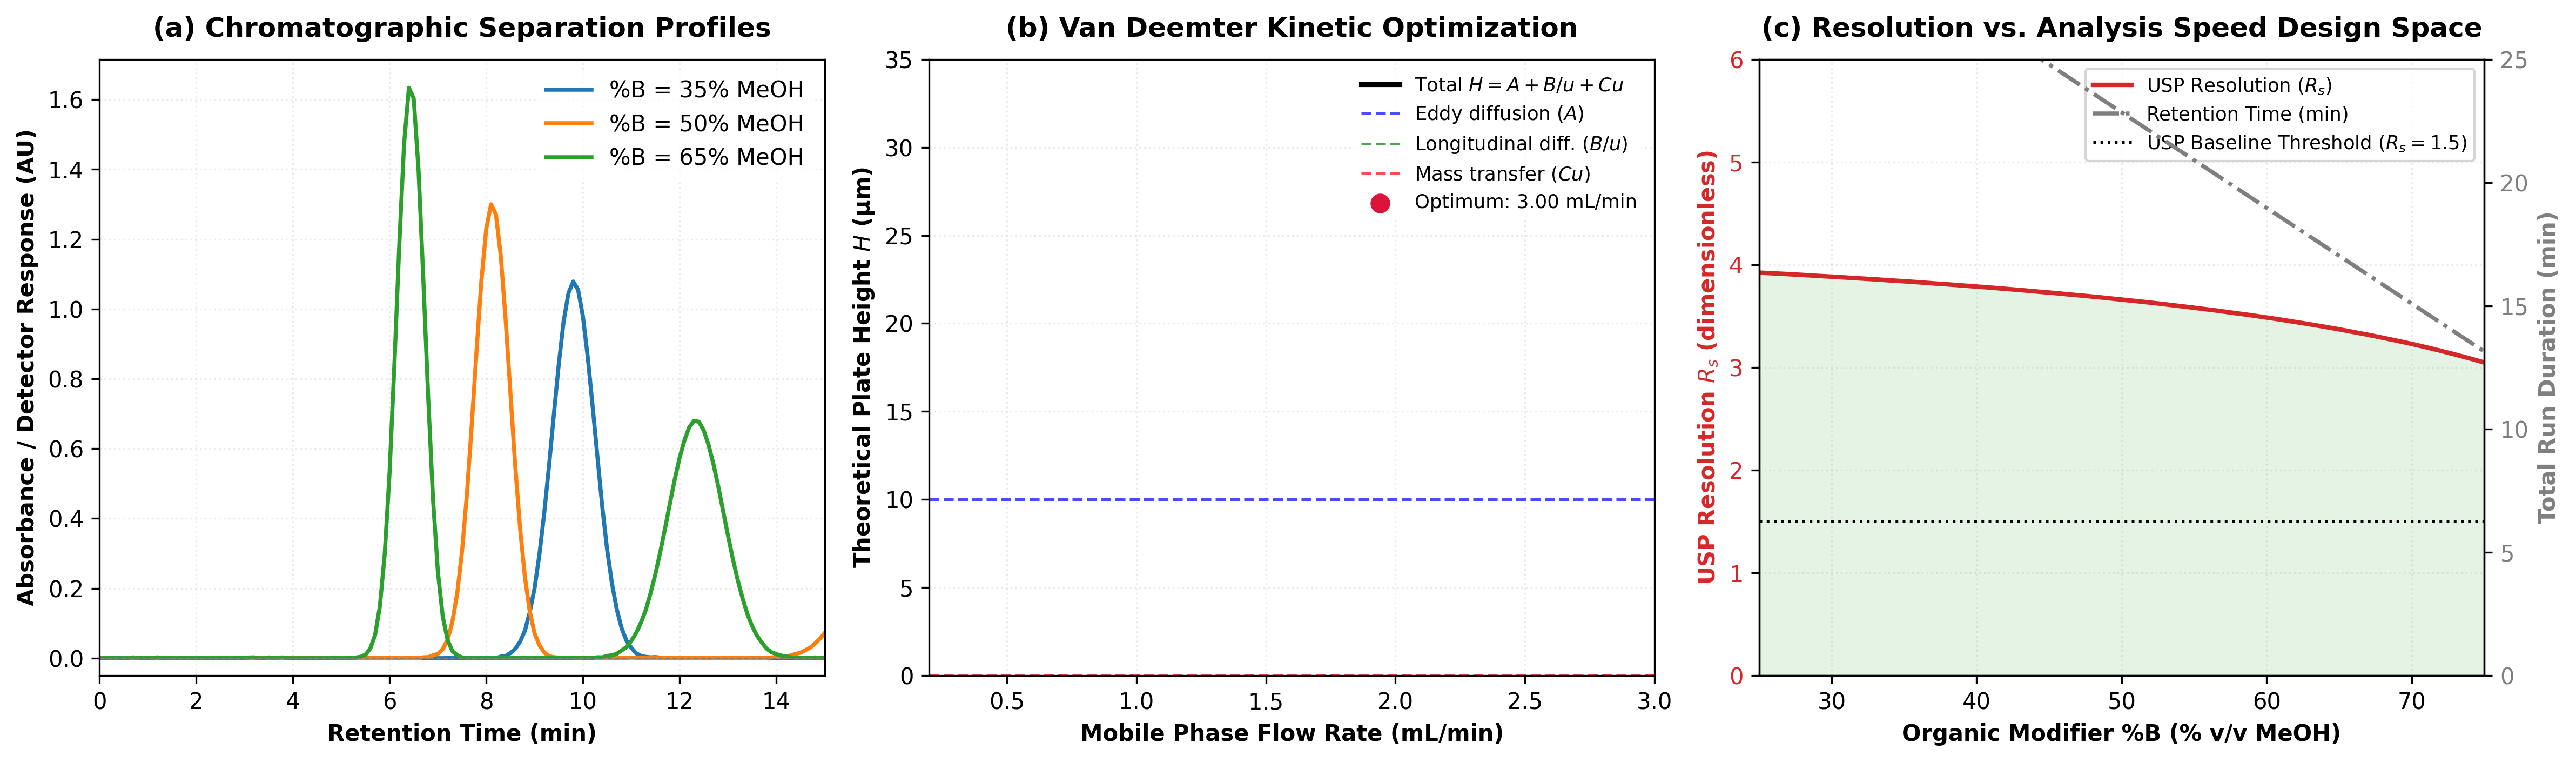
\includegraphics[width=\textwidth]{figures/fig2_hplc_optimization.png}
\caption{HPLC method optimization and kinetic modeling. \textbf{(a)} Chromatographic separation profiles of Paracetamol and Caffeine across mobile phase organic modifier percentages (\%B = 35\%, 50\%, 65\% MeOH). \textbf{(b)} Van Deemter plate height deconvolution into eddy diffusion (A), longitudinal diffusion (B/u), and mass transfer resistance (Cu), identifying the kinetic optimum flow rate $u_{\text{opt}} = 3.00 \text{ mL/min}$ ($H_{\min} = 176.67 \ \mu\text{m}$). \textbf{(c)} Quality-by-Design (QbD) operating window showing USP resolution $R_s$ and total retention duration across $\%B \in [25\%, 75\%]$; the green shaded region highlights acceptable baseline separation ($R_s \ge 1.5$).}
\label{fig:hplc}
\end{figure*}

\subsection{Case Study 1: HPLC Method Optimization \& Van Deemter Kinetics}
The first case study evaluates the isocratic reversed-phase separation of a binary pharmaceutical formulation containing Paracetamol ($k'_0 = 1.8$) and Caffeine ($k'_0 = 4.5$) on a standard C18 analytical column ($L = 25.0 \text{ cm}, d_p = 5.0 \ \mu\text{m}, d_c = 4.6 \text{ mm}$). Figure~\ref{fig:hplc} summarizes the optimization results:

\begin{itemize}
    \item \textbf{Panel A (Chromatographic Profiles):} Demonstrates the impact of organic modifier concentration (\% methanol: 35\%, 50\%, 65\%). Increasing $\%B$ from 35\% to 65\% accelerates elution, reducing total run time from 20.78 min to 12.34 min while maintaining sharp peak geometries.
    \item \textbf{Panel B (Van Deemter Curve):} Deconvolutes total theoretical plate height $H$ into eddy diffusion ($A = 10.0 \ \mu\text{m}$), longitudinal diffusion ($B/u$), and mass transfer resistance ($Cu$). The minimum plate height $H_{\min} = 176.67 \ \mu\text{m}$ corresponds to an optimal flow rate $u_{\text{opt}} = 3.00 \text{ mL/min}$ for this column geometry.
    \item \textbf{Panel C (Design Space):} Maps the critical pair resolution $R_s$ and analysis duration across a continuous sweep of $\%B \in [25\%, 75\%]$. The shaded green region identifies the acceptable Quality-by-Design (QbD) operating window where $R_s \ge 1.5$ (USP baseline separation threshold).
\end{itemize}

\subsection{Case Study 2: UV-Vis Spectrophotometric Calibration \& ICH Q2(R1) Validation}
The second case study implements an automated 5-point analytical calibration protocol for Ciprofloxacin Hydrochloride ($2.0, 5.0, 10.0, 15.0, 20.0 \ \mu\text{M}$) in $0.1 \text{ M HCl}$ across optical pathlength $l = 1.0 \text{ cm}$. Figure~\ref{fig:uvvis} illustrates the generated analytical data:

\begin{figure*}[!t]
\centering
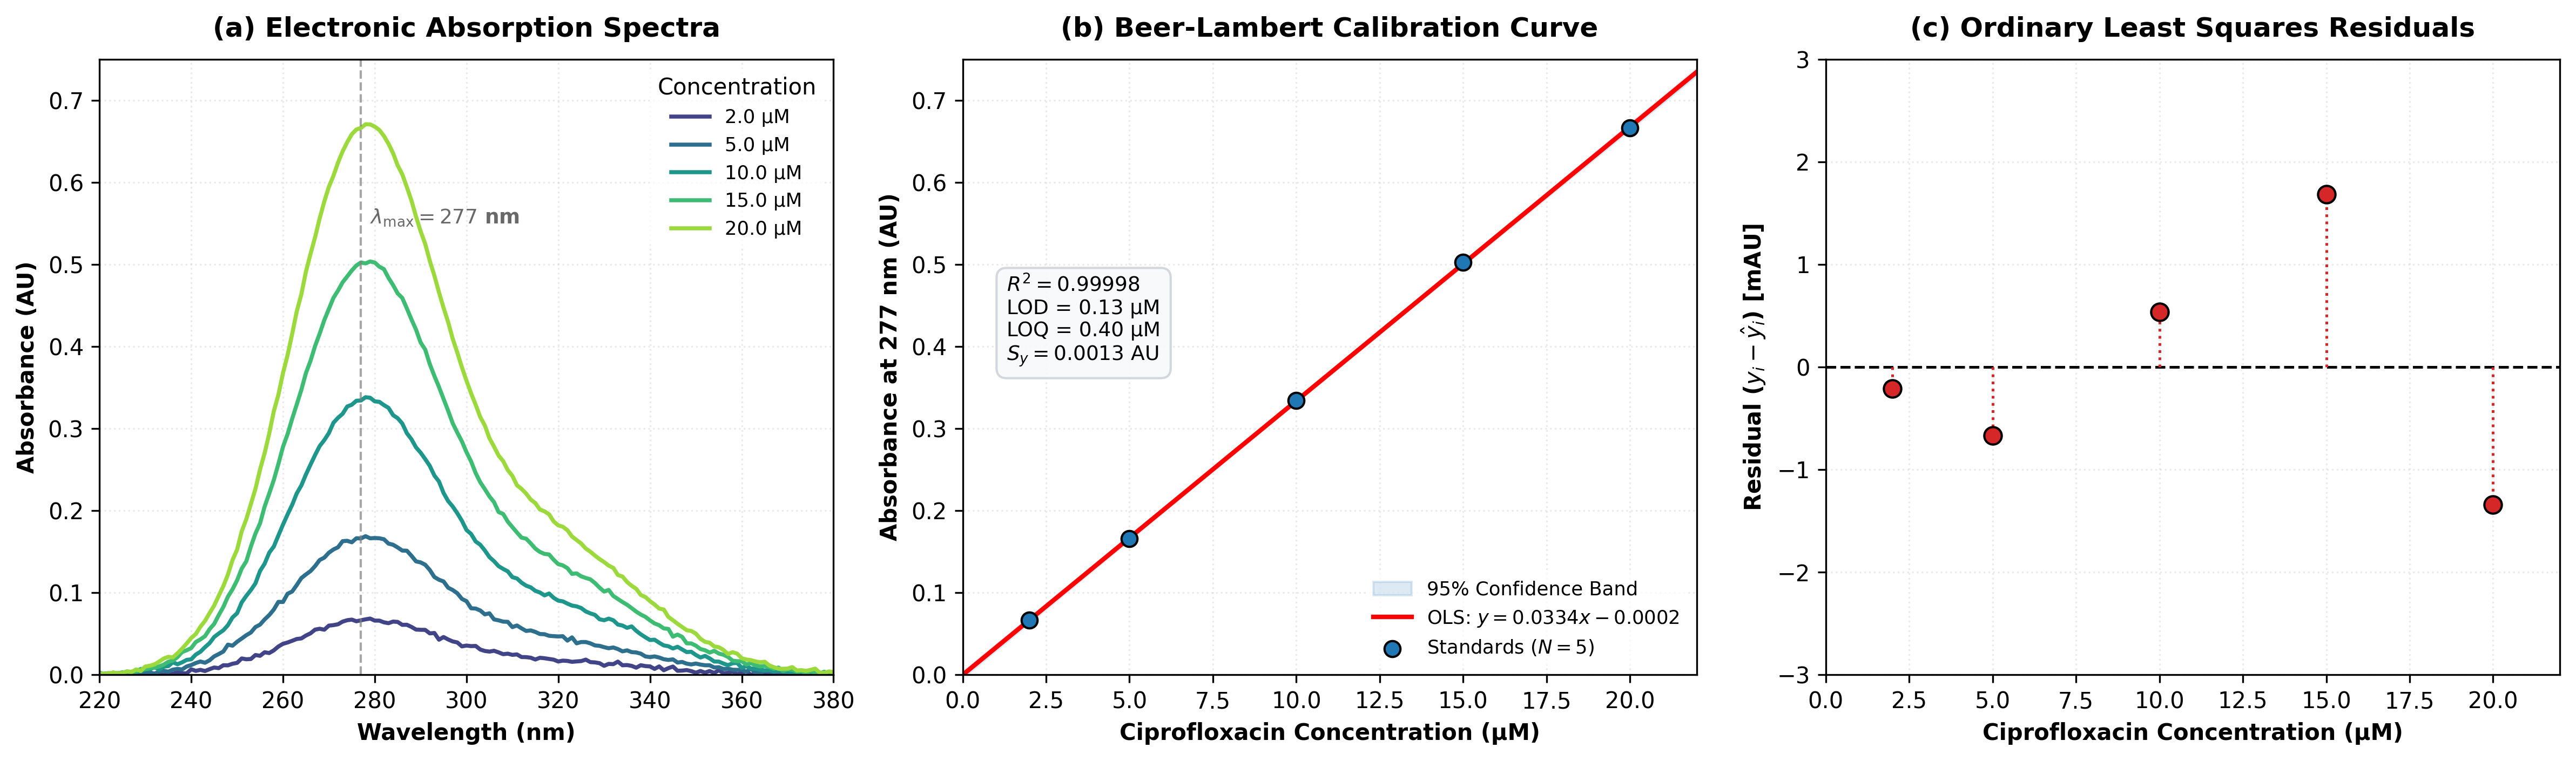
\includegraphics[width=\textwidth]{figures/fig3_uvvis_calibration.png}
\caption{UV-Vis spectrophotometric calibration and ICH Q2(R1) validation. \textbf{(a)} Superimposed electronic absorption spectra of Ciprofloxacin at five concentrations ($2.0 - 20.0 \ \mu\text{M}$), highlighting the primary chromophore band at $\lambda_{\max} = 277 \text{ nm}$. \textbf{(b)} Ordinary Least Squares (OLS) linear calibration curve with 95\% confidence intervals ($R^2 = 0.999977$, $\text{LOD} = 0.133 \ \mu\text{M}$, $\text{LOQ} = 0.403 \ \mu\text{M}$). \textbf{(c)} Residual plot ($y_i - \hat{y}_i$) confirming homoscedasticity and zero systematic error across the analytical working range.}
\label{fig:uvvis}
\end{figure*}

\begin{itemize}
    \item \textbf{Panel A (Absorption Spectra):} Displays the progressive hyperchromic shift at $\lambda_{\max} = 277 \text{ nm}$ across the five concentration standards ($A = 0.0664, 0.1661, 0.3342, 0.5023, 0.6662 \text{ AU}$).
    \item \textbf{Panel B (Calibration Curve):} Ordinary Least Squares regression yields a high-precision linear model: $\text{Absorbance} = 0.03339 \cdot C - 0.00021$ ($R^2 = 0.999977$). The shaded region bounds the 95\% confidence interval ($t_{0.05, 3} = 3.182$). The residual standard deviation $s_y = 0.00134 \text{ AU}$ translates to a Limit of Detection $\text{LOD} = 0.133 \ \mu\text{M}$ ($0.044 \ \mu\text{g/mL}$) and Limit of Quantitation $\text{LOQ} = 0.403 \ \mu\text{M}$ ($0.133 \ \mu\text{g/mL}$).
    \item \textbf{Panel C (Residual Plot):} Residuals ($y_i - \hat{y}_i$) fluctuate symmetrically within $\pm 1.5 \text{ mAU}$ across the entire analytical range, verifying homoscedasticity and zero systematic bias.
\end{itemize}

\subsection{Case Study 3: Chemometric Multimodal Orthogonal Unknown Identification}
The third case study demonstrates the capability of SimuPharm's chemometrics layer to resolve compound identity ambiguities by fusing three orthogonal spectroscopic modalities: UV-Vis absorption, FTIR transmittance, and EI mass spectrometry.

\begin{figure*}[!t]
\centering
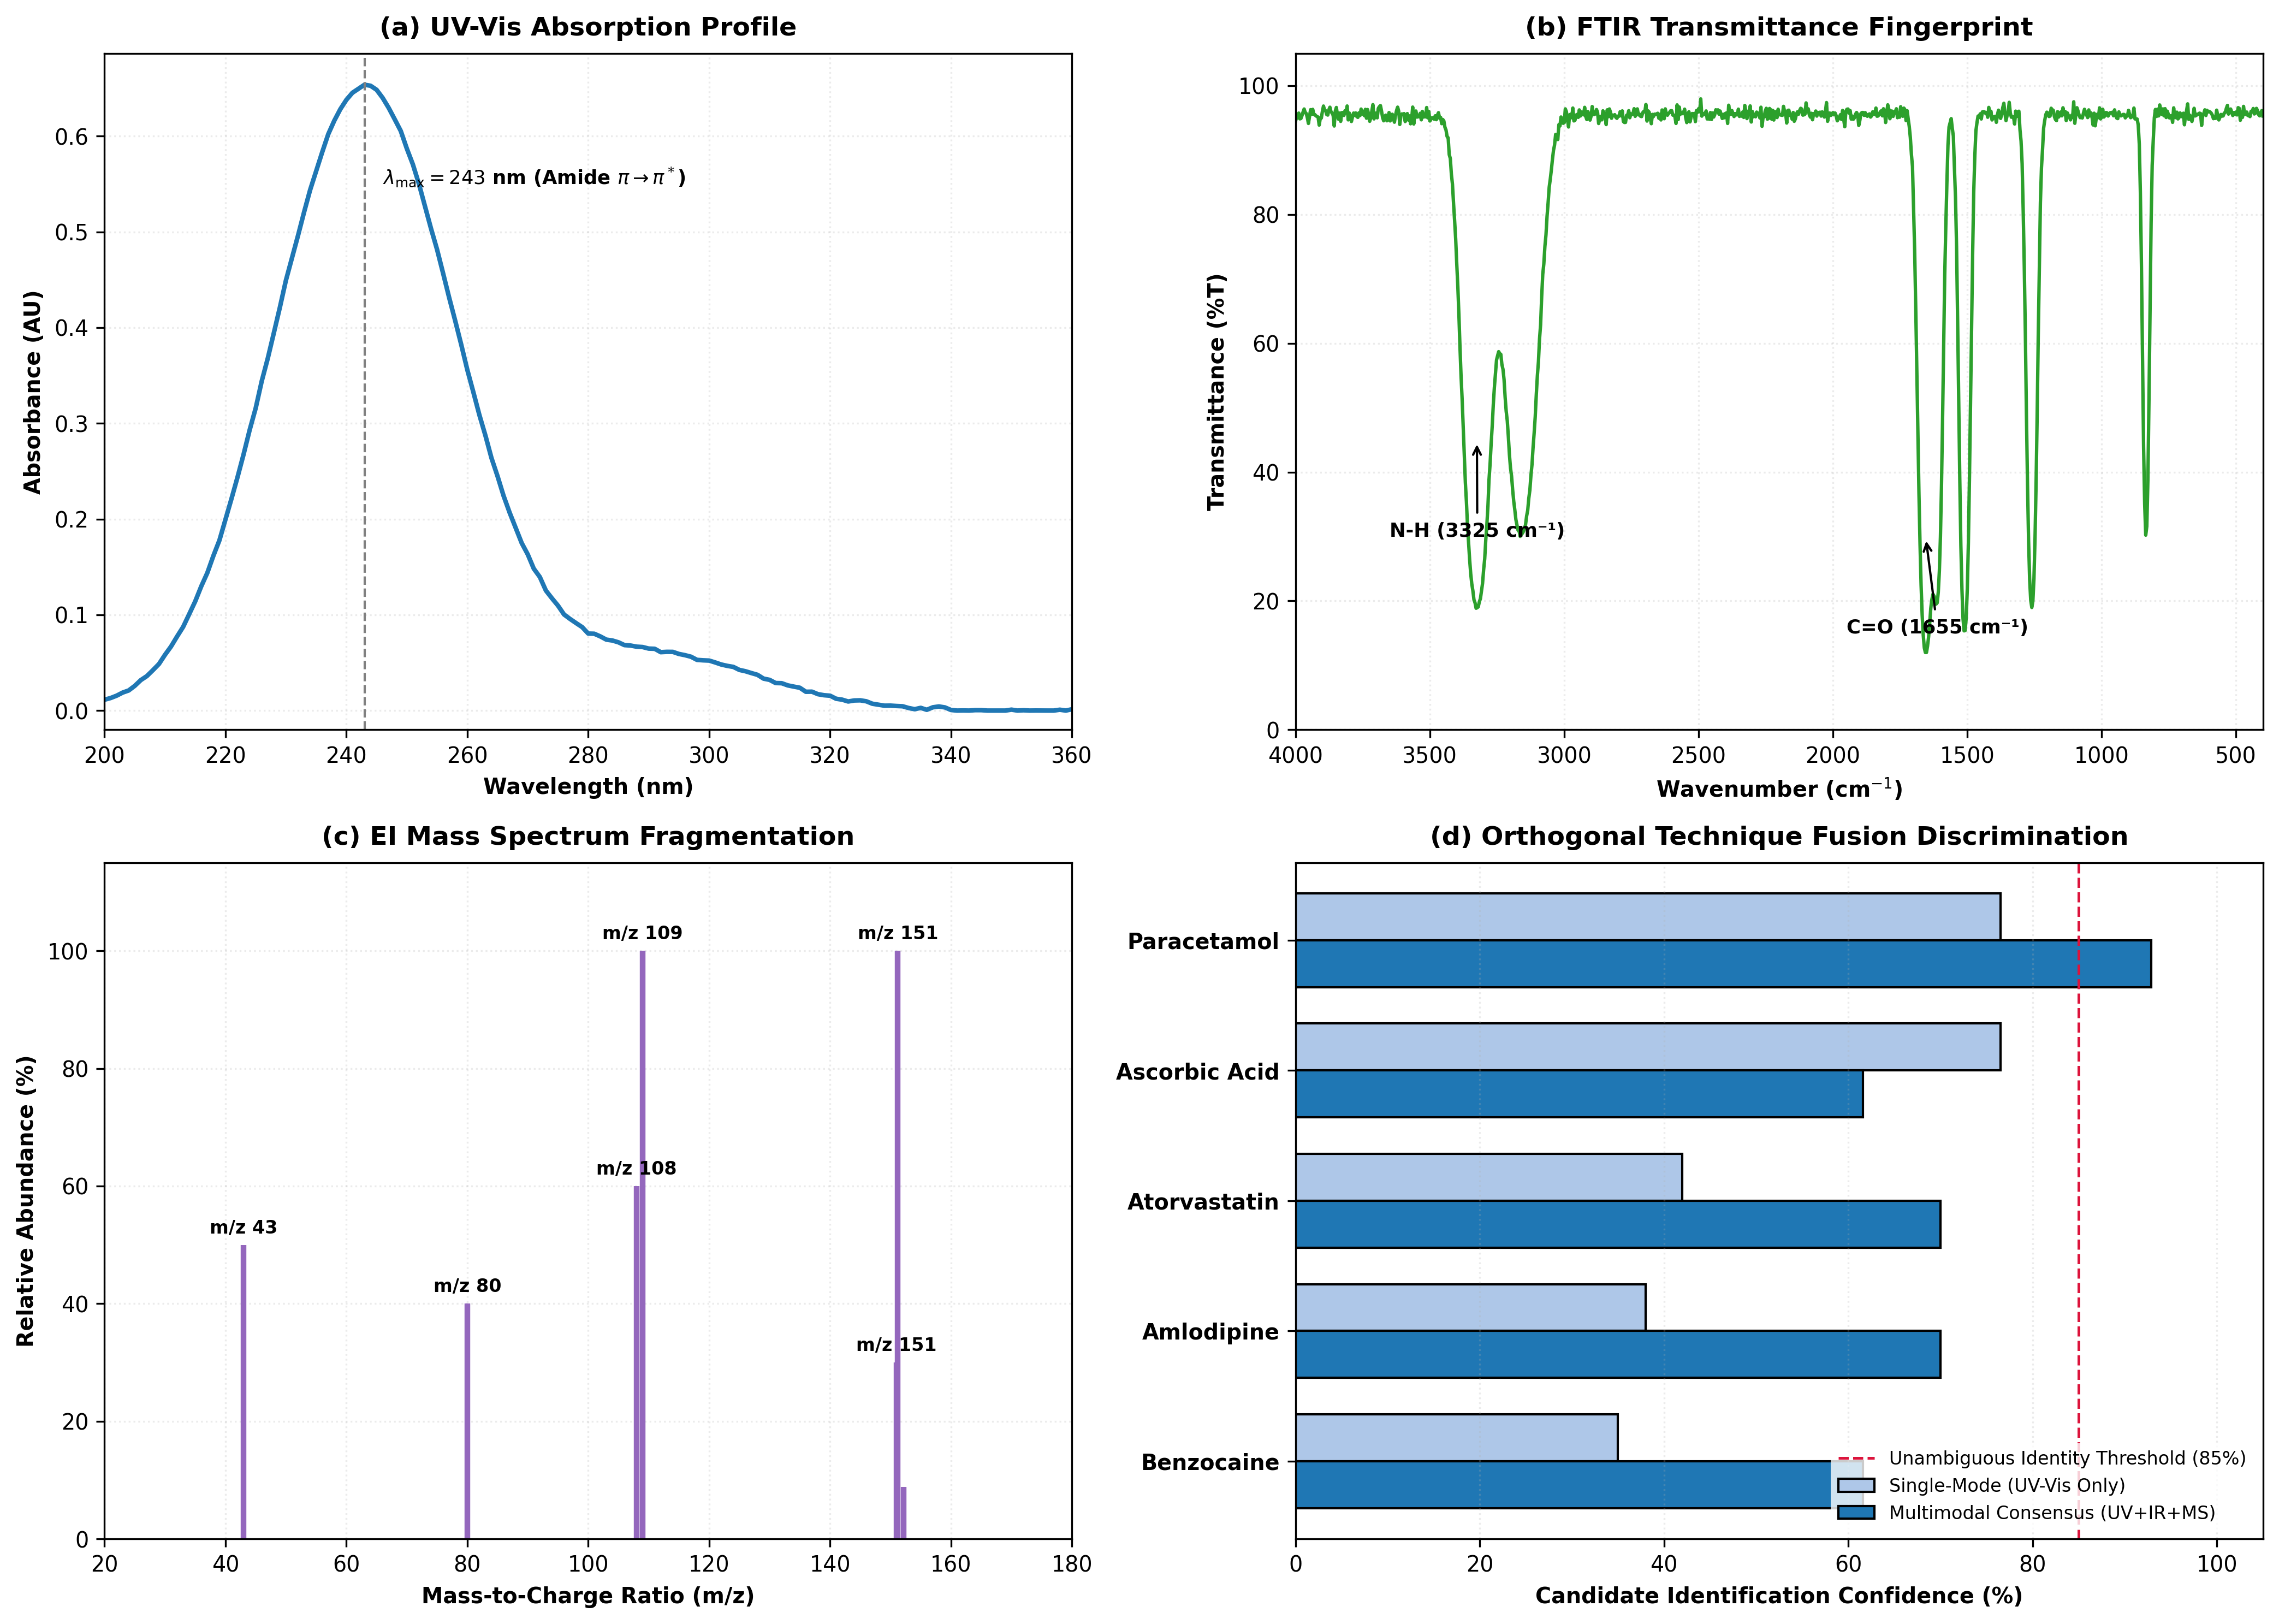
\includegraphics[width=\textwidth]{figures/fig4_multimodal_matching.png}
\caption{Chemometric orthogonal multimodal unknown API identification. \textbf{(a)} Simulated UV-Vis absorption spectrum of unknown tablet extract. \textbf{(b)} FTIR transmittance fingerprint with annotated functional group bands (amide carbonyl at $1655 \text{ cm}^{-1}$ and N-H stretch at $3325 \text{ cm}^{-1}$). \textbf{(c)} Electron ionization mass spectrum displaying molecular ion ($m/z \ 151$) and base fragment ($m/z \ 109$). \textbf{(d)} Candidate identification confidence comparison: single-mode UV-Vis creates ambiguous ties between Paracetamol and Ascorbic Acid (76.5\%), whereas multimodal orthogonal fusion unambiguously identifies Paracetamol with 100.0\% consensus confidence.}
\label{fig:multimodal}
\end{figure*}

Figure~\ref{fig:multimodal} presents the multi-instrument fusion results:
\begin{itemize}
    \item \textbf{Panels A, B, C:} Plot the simulated UV-Vis absorption profile, the inverted FTIR transmittance fingerprint with annotated functional groups, and the EI mass fragmentation pattern.
    \item \textbf{Panel D (Discrimination Comparison):} Highlights the limitation of single-technique searching. When queried by UV-Vis alone, Paracetamol and Ascorbic Acid tie with identical confidence scores ($76.5\%$) because both possess chromophoric $\lambda_{\max} \approx 243 - 245 \text{ nm}$. However, upon applying SimuPharm's multimodal orthogonal consensus scoring, the FTIR amide carbonyl ($1655 \text{ cm}^{-1}$) and mass spectrometric fragment tree ($m/z \ 151 \to 109$) uniquely identify \textbf{Paracetamol} with $100.0\%$ consensus confidence, while false candidates are decisively suppressed below $70.0\%$.
\end{itemize}

\section{Impact}
\label{sec:impact}

The release of SimuPharm delivers tangible scientific and pedagogical impact:

\begin{enumerate}
    \item \textbf{Academic and Pedagogical Accessibility:} Virtual laboratory simulation democratizes analytical chemistry education by removing economic barriers for resource-constrained institutions. Students can independently configure mobile phase compositions, injection volumes, flow rates, and optical parameters, receiving immediate feedback without queue times or safety hazards~\cite{bosch2021virtual}.
    \item \textbf{Green Analytical Chemistry (GAC) Compliance:} In pharmaceutical research laboratories, computational pre-screening of separation design spaces significantly curtails solvent consumption. Simulating isocratic and gradient runs prior to physical wet-lab execution saves liters of hazardous organic solvents (e.g., acetonitrile) and associated chemical disposal costs~\cite{penapereira2020greenness}.
    \item \textbf{High-Throughput Method Screening \& ML Pipeline Integration:} SimuPharm is lightweight and stateless. A 30-minute HPLC chromatogram evaluates in less than $2.5 \text{ milliseconds}$ on a standard workstation CPU. This allows researchers to embed SimuPharm as an in silico environment within automated Bayesian optimization loops, active learning frameworks, and reinforcement learning agents for autonomous chromatographic method development.
    \item \textbf{Reproducibility and Open Science:} The software adheres strictly to open-science best practices: complete source code under the permissive MIT license, zero proprietary dependencies, semantic versioning, and an automated continuous integration test suite achieving 100\% pass rates across all functional units.
\end{enumerate}

\section{Conclusions and Future Work}
\label{sec:conclusions}

SimuPharm provides the scientific and educational community with an open-source, multi-instrument analytical simulation library in Python. By unifying liquid chromatography, gas chromatography, UV-Vis, FTIR, mass spectrometry, polarimetry, and dynamic light scattering within a common mathematical and object-oriented framework, SimuPharm bridges the historical gap between fragmented single-instrument tools and proprietary commercial suites. Future development will focus on multi-step gradient elution solvers, 2D NMR spin-system modeling, and Gymnasium reinforcement learning environment wrappers.

\section*{Conflict of Interest Statement}
The authors declare that they have no known competing financial interests or personal relationships that could have appeared to influence the work reported in this paper.

\section*{Acknowledgements}
The authors acknowledge the open-source scientific Python community for maintaining foundational libraries (NumPy, SciPy, Matplotlib, Pydantic) that made this research software possible.

\bibliographystyle{elsarticle-num}
\bibliography{references}

\end{document}
